\documentclass[11pt,a4paper]{article}
\usepackage[top=2.5cm, bottom=2cm, left=2cm, right=2cm]{geometry}
\usepackage{amsmath}
\usepackage{tikz}
\usepackage{circuitikz}
\usepackage{epigraph}
\usepackage{hyperref}
\usepackage{multirow}
%\usepackage[demo]{graphicx}
\usepackage{caption}
\usepackage{subcaption}
\setcounter{secnumdepth}{5}
\usepackage{chngcntr}
\counterwithin{figure}{section}
\counterwithin{table}{section}
\usepackage{multirow}
\setcounter{tocdepth}{5}
\usepackage{subfiles}
\usepackage{epstopdf}


% pseudocode
\usepackage{algorithm}
\usepackage[noend]{algpseudocode}


\renewcommand\epigraphflush{flushright}
\renewcommand\epigraphsize{\normalsize}
\setlength\epigraphwidth{0.7\textwidth}

\usepackage{color}
\definecolor{titlepagecolor}{cmyk}{1,.0,0.0,.50}
\definecolor{scolour}{cmyk}{1,.0,0.0,.85}
\definecolor{sscolour}{cmyk}{1,.0,0.0,.75}
\definecolor{ssscolour}{cmyk}{1,.0,0.0,.65}
\definecolor{paracolour}{cmyk}{1,.0,0.0,.55}

\usepackage{amsfonts}
%\DeclareFixedFont{\titlefont}{T1}{ams}{b}{sc}{0.5in}

% Added 
\usepackage{fancyhdr}
\pagestyle{fancy}
\lhead{AERO4701}
\rhead{Assignment 1}
\cfoot{\thepage}
\renewcommand{\headrulewidth}{0.4pt}
\renewcommand{\footrulewidth}{0.4pt}
\renewcommand{\thepage}{\roman{page}}
\usepackage{indentfirst}           %remove if we dont want to indent
\renewcommand{\thepage}{\roman{page}}

\newcommand{\myparagraph}[1]{\paragraph{#1}\mbox{}\newline\indent}
% vectors
\newcommand{\dv}[1]{\textbf{\textit{#1}}}
\newcommand{\vv}[1]{\dot{\textbf{\textit{#1}}}}
\newcommand{\av}[1]{\ddot{\textbf{\textit{#1}}}}

\newlength{\normalparindent}
\AtBeginDocument{\setlength{\normalparindent}{\parindent}}

% Change heading colours
\usepackage{titlesec}
%\usepackage[usenames,dvipsnames]{xcolor}
\usepackage{bold-extra}
\titleformat{\section}
{\color{scolour}\scshape\LARGE\bfseries}
{\color{scolour}\thesection.}{2em}{}
\titleformat{\subsection}
{\color{sscolour}\normalfont\Large\bfseries}
{\color{sscolour}\thesubsection}{2em}{}
\titleformat{\subsubsection}
{\color{ssscolour}\normalfont\large\bfseries}
{\hspace*{\normalparindent}\color{ssscolour}\thesubsubsection}{1em}{}
\titleformat{\paragraph}
{\color{paracolour}\normalfont\large\bfseries}
{\hspace*{\normalparindent}\color{paracolour}\theparagraph}{1em}{}

% end added
\makeatletter                       
\def\printauthor{%                  
    {\large \@author}}              
\makeatother
\author{%
    Lydia Drabsch \\
    311217591 \\
    \texttt{ldra3557@uni.sydney.edu.au}\vspace{20pt} 
    \\
    }


% Title image
\newcommand\titlepagedecoration{%
\tikz[remember picture,overlay] \node[opacity=1,inner sep=0pt] at ([xshift=5cm]current page.west){
\includegraphics[height=\paperheight]{./IMAGEtitle2f}};
}

% Matlab Code
\usepackage[framed]{mcode}

\begin{document}
\newgeometry{top=3.7cm, bottom=4cm, left=3cm, right=3cm}

\begin{titlepage}
\titlepagedecoration

\flushright
\huge{\scshape Space Engineering 3}\\ Assignment 1 \\ 24th March 2016


\null\vfill
%\vspace{2cm}
\begin{minipage}{0.8\textwidth}
\centering
\rule{1\textwidth}{0.02pt}\\
\Huge{\textbf{\scshape Orbit Simulation and Determination}\\\rule{1\textwidth}{0.02pt}}
\\ 
\end{minipage}


\null\vfill
\vspace*{1cm}
\noindent
\hfill
\begin{minipage}{0.45\linewidth}
    \begin{flushright}
        \printauthor
    \end{flushright}
\end{minipage}
%
\begin{minipage}{0.02\linewidth}
    \rule{1pt}{60pt}
\end{minipage}


\end{titlepage}
\newgeometry{top=2.5cm, bottom=2cm, left=2cm, right=2cm}

\begin{figure*}[h!]
\centering
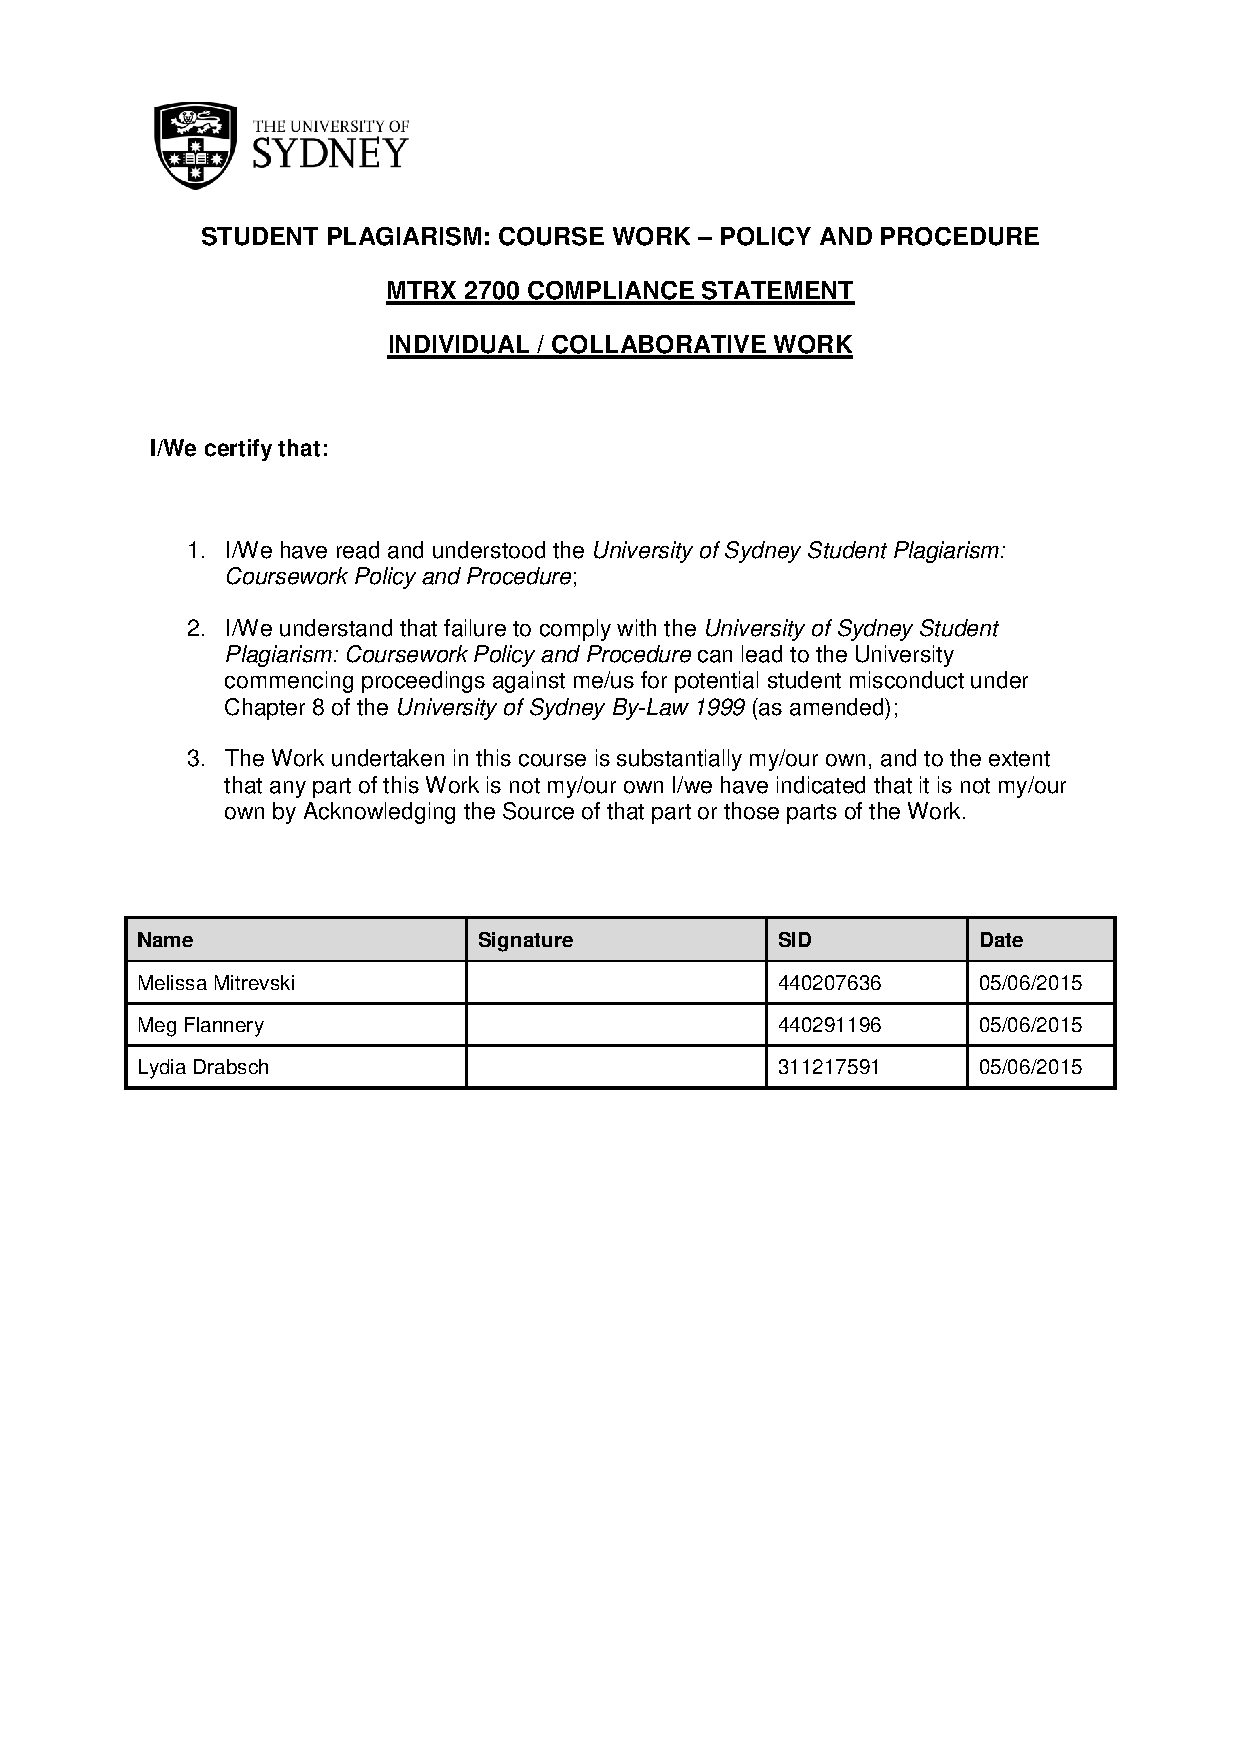
\includegraphics[width=0.99\linewidth]{./Plag}
\label{fig:Plag}
\end{figure*}

\setcounter{section}{0}

\tableofcontents
\listoffigures
\listoftables
\newpage
\pagenumbering{arabic}
%\renewcommand{\thepage}{\arabic{page}}




\section*{Introduction}
Each mainQN.m file has a section called 'User Input' where the animations and state plots can be turned on/off. Also the timestep and the number of days to simulate are defined. The default settings are dt = 100 seconds and days = 1.

\subfile{Ques1}


\subfile{Ques2}


\subfile{Ques3}



\section{Conclusions}

\newpage
\bibliographystyle{IEEEtran}
\bibliography{file}


\newpage
\section{Appendix}

\end{document}